\documentclass{beamer}
\setbeamercovered{transparent}

\usepackage{epstopdf}
\usepackage[inline]{asymptote}

\mode<presentation> %?

\usetheme{Frankfurt}
\usepackage{helvet}
\usepackage{mathptmx}
%\usefonttheme{professionalfonts}
\usefonttheme[onlymath]{serif}
\usefonttheme{structurebold}

%\renewcommand{\familydefault}{Futura}
%\setsansfont{Verdana}

\setlength{\unitlength}{\paperwidth}

% width, height, title, content
\newcommand{\SizedBlock}[4]{
  \begin{block}{#3}
    \parbox[t][#2\paperwidth][t]{#1\paperwidth}{#4}    
  \end{block}
}

% w1, c1, w2, c2
\newcommand{\TwoColumns}[4]{
  \vspace{-0.02\paperwidth}
  \begin{columns}[t]
    \begin{column}{#1\paperwidth}
      #2
    \end{column}\hspace{-0.02\paperwidth}
    \begin{column}{#3\paperwidth}
      #4
    \end{column}
  \end{columns}
}

% w1, c1, w2, c2, w3, c3
\newcommand{\ThreeColumns}[6]{
  \vspace{-0.02\paperwidth}
  \begin{columns}[t]
    \begin{column}{#1\paperwidth}
      #2
    \end{column}\hspace{-0.07\paperwidth}
    \begin{column}{#3\paperwidth}
      #4
    \end{column}\hspace{-0.07\paperwidth}
	\begin{column}{#5\paperwidth}
      #6
    \end{column}
  \end{columns}
}

% height, title1, content1, title2, content2
\newcommand{\TwoColumnBlocksW}[6]{
  \TwoColumns{
        #6}{
        \SizedBlock{#6}{#1}{#2}{#3}}{
        #6}{
        \SizedBlock{#6}{#1}{#4}{#5}}
}

% height, title1, content1, title2, content2
\newcommand{\TwoColumnBlocks}[5]{
  \TwoColumnBlocksW{#1}{#2}{#3}{#4}{#5}{0.4}
}

% height, title1, content1, title2, content2, title3, content3
\newcommand{\ThreeColumnBlocks}[7]{
  \ThreeColumns{
        0.24}{
        \SizedBlock{0.24}{#1}{#2}{#3}}{
        0.24}{
        \SizedBlock{0.24}{#1}{#4}{#5}}{
        0.24}{
        \SizedBlock{0.24}{#1}{#6}{#7}}
}

\newcommand{\PutPic}[3]{
  \put(#1){\includegraphics[#2\paperwidth]{./img/#3}}
}

\usepackage{color}

\begin{document}
\title{Sphere Mesh: shape approximation using sphere quadric error metrics}
\author{Tengfei Jiang}

\newcommand{\FPP}[2]{\frac{\partial #1}{\partial #2}}
\begin{frame}
  \titlepage
\end{frame}

\begin{frame}{Outline}
\begin{itemize}
\item Background
\item Key Problem
\item Solution
\item Results
\item Conclusion
\end{itemize}
\end{frame}

\begin{frame}{Background}
\begin{block}{Motivation}
Mesh simplifications
\begin{itemize}
\item Clustering methods
\item Decimation methods (QEM)
\item Resampling methods
\item Simplification of volumetric structure
\end{itemize}
\end{block}
Sphere Mesh representing structure
\end{frame}

\begin{frame}{Key Problem}
\begin{itemize}
\item Where to put a sphere?
\item What's the radius of each sphere?
\item How to connect these spheres?
\end{itemize}
\end{frame}


\begin{frame}{Solutions}
\begin{block}{Sphere Mesh representation}
$\{S,E,T\}$ stands for sphere $S_i=(q_i,r_i)$, edges, triangles.\\
Implicit surface: sphere is interpolated along edge and triangle.
\end{block}
\begin{figure}
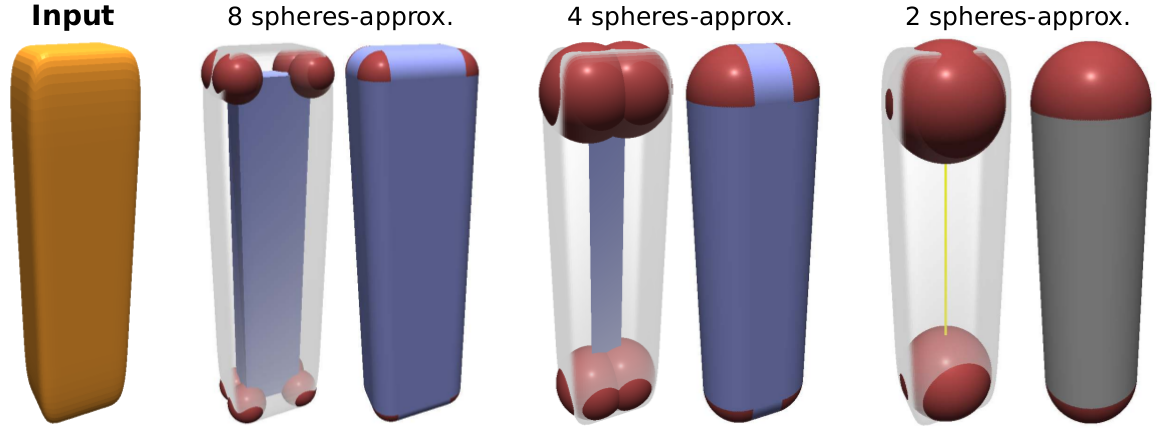
\includegraphics[height=1.5in]{./img/representation.png}
\end{figure}
\end{frame}

\begin{frame}{Sphere Quadric Error Metric (SQEM)}
Signed Distance:
\[d(S_i,Plane)=n^t.(p-q)-r\]
\begin{figure}
\vspace{-4mm}
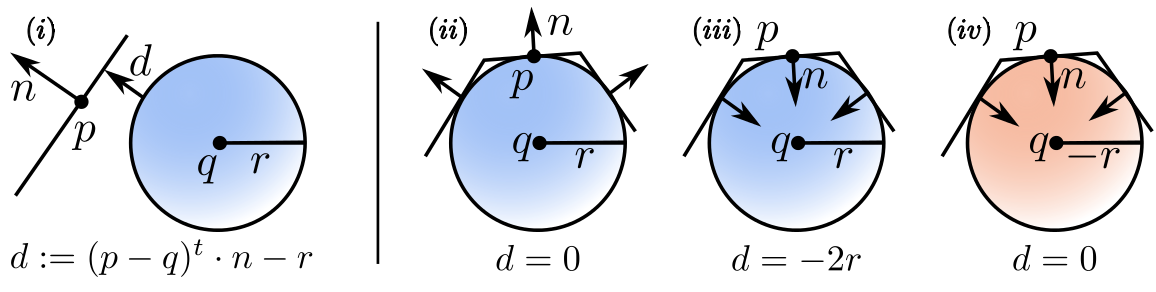
\includegraphics[height=0.8in]{./img/distance.png}
\end{figure}
SQEM:
\begin{eqnarray}
SQEM_i(s) = d^2 = Q(s) = \frac{1}{2}s^TAs-b^ts+c
\end{eqnarray}
\end{frame}

\begin{frame}{Shape Approximation}
Partition input mesh to regions (vertex groups) $P_{I_k}$, each region is approximated by one sphere.
Approximation error:
\begin{eqnarray}
\sum_k \int_{v\in P_{I_k}} Q(s_k) dv
\end{eqnarray}
In discretization:
\TwoColumns{0.4}{
\[Q(s_k)=\sum_{t_j\in T}\frac{Area_{t_j}}{3}d(s_k,t_j)^2\]
}{0.4}{
\begin{figure}
\vspace{-4mm}
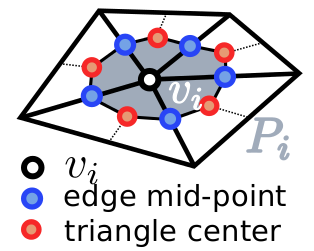
\includegraphics[height=1.0in]{./img/dis.png}
\end{figure}
}
\end{frame}

\begin{frame}{Mesh Simplification}
Edge collapsion guided by SQEM:
\begin{itemize}
\item For edge $uv$, $min\: Q_u(s) + Q_v(s)$
\item Add edge $uv, s, Q_u+Q_v$ into a queue $\mathcal{Q}$
\item Collapse edge based on $\mathcal{Q}$ until sphere number satisify user's requirements
\end{itemize}
\end{frame}

\begin{frame}{Q.A}
\end{frame}
\end{document}
